\chapter{Introducción específica} 

\label{Chapter2}

Este capítulo presenta los conceptos y componentes centrales que sustentan el trabajo. Se introducen los sistemas de recomendación y sus enfoques principales, se describen las fuentes de información empleadas y se detallan las plataformas y herramientas utilizadas para el procesamiento de datos, el modelado y la gestión de experimentos, que conforman la base tecnológica de la solución propuesta.
%----------------------------------------------------------------------------------------

\section{Sistemas de recomendación}

Los sistemas de recomendación constituyen una de las aplicaciones más extendidas de la inteligencia artificial, con un papel central en la reducción de la sobrecarga de información y en la optimización de decisiones de consumo. Su finalidad es generar sugerencias personalizadas que se ajusten a las características de cada cliente, lo que incrementa la relevancia de los productos ofrecidos y mejora la experiencia general de interacción con la empresa.

\subsection{Funcionamiento de los sistemas de recomendación}

El eje central del enfoque consiste en identificar relaciones de similitud en los datos disponibles. Estas relaciones pueden establecerse desde diferentes perspectivas. En primer lugar, es posible medir la similitud entre productos, lo que permite agrupar aquellos que suelen adquirirse en conjunto o que comparten atributos comunes. En segundo lugar, puede analizarse la similitud entre clientes, de modo que las preferencias observadas en un grupo con comportamientos semejantes permitan anticipar las elecciones de otros con perfiles cercanos. Por último, también resulta clave la similitud entre interacciones, que considera el historial de comportamientos de un cliente, como sus compras o búsquedas, para anticipar futuras decisiones.

Un ejemplo ilustrativo, representado en la figura \ref{fig:ejemploSimilitud}, puede plantearse en la industria de bebidas. Supongamos que cada marca de cerveza se representa como un vector en un espacio definido por atributos, como “tradicional versus innovador” y “masivo versus \textit{premium}”. En ese espacio, una lager clásica de gran consumo quedaría ubicada cerca de otras variedades tradicionales y de alcance masivo, mientras que una IPA artesanal o una edición limitada se situarían en la región asociada a lo \textit{premium} e innovador. El sistema de recomendación aprovecha esta representación para calcular distancias o similaridades entre productos. Si un cliente suele elegir artículos situados en torno al cuadrante de “\textit{premium}–tradicional”, el modelo infiere que probablemente muestre interés por otras marcas que ocupan posiciones cercanas en ese mismo espacio vectorial. De esta manera, la proximidad entre vectores se convierte en un indicador de afinidad, que guía la generación de recomendaciones personalizadas.

\begin{figure}[htpb]
	\centering
	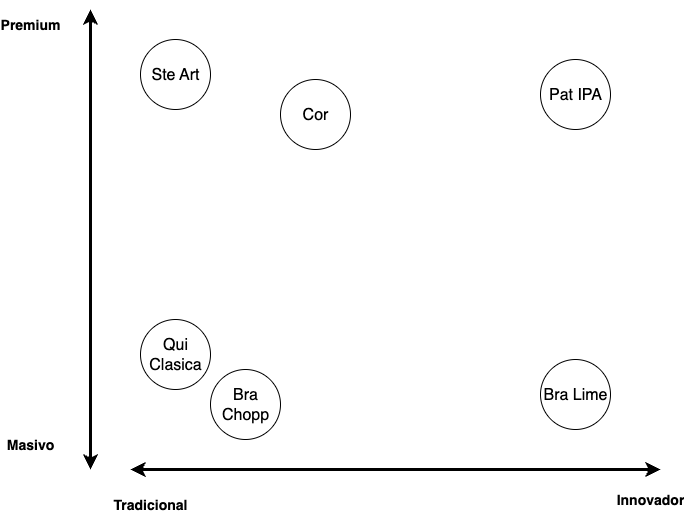
\includegraphics[scale=.4]{./Figures/ejemploSimilitud.png}
	\caption{Ejemplo de representación de marcas de cerveza en un espacio de atributos.}
	\label{fig:ejemploSimilitud}
\end{figure}

\subsection{Tipos de \textit{feedback}}

El tipo de información disponible para alimentar un sistema de recomendación también es determinante. Se distinguen dos formas principales de retroalimentación. La retroalimentación explícita consiste en la valoración directa que realizan los clientes sobre los productos, como calificaciones numéricas, encuestas o reseñas. La retroalimentación implícita, en cambio, se infiere del comportamiento de los clientes, ya sea a través de sus compras, búsquedas o interacciones digitales. En el ámbito B2B, donde no es común que los clientes asignen calificaciones explícitas, predominan las señales implícitas, lo que plantea desafíos adicionales para la construcción de modelos precisos.

\subsection{Filtrado colaborativo}

Entre los enfoques más utilizados se encuentra el filtrado colaborativo, que parte de la hipótesis de que “usuarios similares tienden a preferir ítems similares”. Este enfoque puede abordarse desde dos variantes principales. En la modalidad \textit{user-based}, se recomienda a un cliente productos que fueron consumidos por otros con patrones de compra semejantes. En la modalidad \textit{item-based}, se priorizan productos que suelen aparecer en conjunto en los historiales de distintos clientes. 

El filtrado colaborativo suele implementarse mediante técnicas de factorización matricial. Dado un conjunto de $m$ usuarios y $n$ productos, se construye una matriz de interacciones $R \in \mathbb{R}^{m \times n}$, donde cada celda refleja el vínculo entre un cliente y un producto. El objetivo consiste en aproximar esta matriz como el producto de dos matrices de menor dimensión:

\begin{equation}
\label{eq:factorizacion}
R \approx U \cdot V^T
\end{equation}

donde $U \in \mathbb{R}^{m \times k}$ representa a los usuarios en un espacio latente de dimensión $k$, y $V \in \mathbb{R}^{n \times k}$ representa a los ítems en ese mismo espacio. La predicción de la afinidad del usuario $i$ con el ítem $j$ se calcula como:

\begin{equation}
\label{eq:prediccion_cf}
\hat{r}_{ij} = u_i \cdot v_j^T
\end{equation}

Este modelo permite capturar relaciones complejas entre clientes y productos a partir de información implícita, aunque presenta limitaciones frente al problema del arranque en frío, cuando no existe historial suficiente de interacciones.

\subsection{Sistemas basados en contenido}

Otro enfoque ampliamente utilizado es el de los sistemas basados en contenido, que centran la recomendación en las características de los productos y en el perfil de cada cliente. En este caso, se representa a cada producto por un vector de atributos y se construye un perfil para cada cliente que refleja la importancia relativa de esos atributos en función de sus elecciones pasadas. La predicción de relevancia para recomendar un producto $j$ a un cliente $i$ puede expresarse de manera simplificada como:

\begin{equation}
\label{eq:prediccion_cb}
\hat{r}_{ij} = w_i \cdot x_j
\end{equation}

donde $x_j$ es el vector de atributos del producto y $w_i$ representa el perfil del cliente. Este método permite recomendar productos nuevos o poco frecuentes siempre que exista información suficiente sobre sus atributos, lo que lo convierte en un complemento natural del filtrado colaborativo.

%----------------------------------------------------------------------------------------

\section{Fuentes de información}

El desarrollo del sistema de recomendación se apoya en un conjunto diverso de datos que, en su integración, permiten construir una representación enriquecida de la relación cliente–producto. Estas fuentes incluyen información transaccional, eventos de interacción en la aplicación BEES y atributos contextuales de clientes y productos. En conjunto, estos elementos aportan evidencia implícita de interés y afinidad, y constituyen la base para la estimación de scores personalizados.

Los datos transaccionales reflejan las compras efectivamente realizadas por cada cliente. Dentro de esta categoría se consideran las siguientes variables: volumen adquirido por producto, frecuencia de compra, recencia de la última operación, monetización total y participación relativa de cada producto en el mix de compras del cliente. Estas medidas permiten capturar el grado de preferencia y relevancia actual de cada artículo en la cartera de cada punto de venta.

A su vez, se incorporan eventos de comportamiento generados en la aplicación BEES, los cuales funcionan como señales implícitas de interés. Entre ellos se incluyen agregados y remociones de productos del carrito, visualizaciones de fichas de producto, búsquedas realizadas, calificaciones o reseñas, y clics en promociones. Estos registros aportan información complementaria sobre el proceso de consideración del cliente, incluso en los casos en los que no se concreta una transacción.

La caracterización se completa con variables de contexto asociadas tanto a clientes como a productos. Del lado del cliente, se integran atributos como el canal comercial y la ubicación geográfica. Del lado del producto, se consideran propiedades como marca, segmento, calibre y participación de mercado. Este conjunto de información contextual permite capturar heterogeneidades relevantes que condicionan la relación de afinidad.

De esta forma, la combinación de datos transaccionales, eventos digitales y atributos contextuales permite construir una representación integral de las interacciones cliente–producto, sobre la cual se sustenta el modelado de afinidad.




%----------------------------------------------------------------------------------------

\section{Herramientas utilizadas}

El desarrollo del trabajo se apoyó en un conjunto de herramientas tecnológicas que permitieron gestionar de manera eficiente el ciclo de vida completo del sistema de recomendación, desde la preparación de datos hasta el despliegue de modelos.

En primer lugar, se utilizó la plataforma \texttt{Databricks}, que combina capacidades de procesamiento distribuido con un entorno colaborativo para el análisis de datos. Databricks permitió integrar múltiples fuentes, realizar transformaciones a gran escala con \texttt{PySpark} y organizar flujos de trabajo de forma reproducible y escalable. Su uso facilitó tanto la exploración inicial como la construcción de pipelines de ingeniería de atributos.

En segundo lugar, se empleó \texttt{MLflow} como herramienta de gestión del ciclo de vida de modelos. A través de esta plataforma se registraron experimentos, parámetros, métricas y versiones de modelos, lo que aseguró trazabilidad y comparabilidad entre distintos enfoques. Asimismo, se utilizaron las funcionalidades de almacenamiento y versionado de artefactos para garantizar la reproducibilidad de resultados y la posibilidad de mantener un repositorio consolidado de modelos entrenados.

El trabajo también se apoyó en librerías de aprendizaje automático ampliamente utilizadas en la comunidad científica y profesional. Entre ellas se destaca \texttt{MLlib}, utilizada para implementar la factorización matricial con \texttt{ALS}. Asimismo, se empleó \texttt{LightFM} para el desarrollo de modelos híbridos de filtrado colaborativo. Finalmente, se incorporó \texttt{PyTorch} como entorno de \textit{deep learning}, lo que permitió construir arquitecturas más complejas capaces de capturar patrones no lineales en las interacciones cliente–producto. Adicionalmente, se utilizaron librerías de visualización como \texttt{matplotlib} y \texttt{seaborn} para generar representaciones gráficas que complementaron el análisis exploratorio y la evaluación de resultados.

Finalmente, se recurrió a entornos de control de versiones y colaboración, en particular \texttt{GitHub}, lo que permitió organizar el código en repositorios estructurados, registrar cambios de manera sistemática y facilitar la integración de componentes en distintas fases del trabajo.

En conjunto, estas herramientas proporcionaron una infraestructura sólida para desarrollar, evaluar y documentar el sistema de recomendación, lo que aseguró tanto la calidad técnica como la escalabilidad del enfoque implementado.


%----------------------------------------------------------------------------------------


% \section{Estilo y convenciones}
% \label{sec:ejemplo}

% \subsection{Uso de mayúscula inicial para los título de secciones}

% Si en el texto se hace alusión a diferentes partes del trabajo referirse a ellas como capítulo, sección o subsección según corresponda. Por ejemplo: ``En el capítulo \ref{Chapter1} se explica tal cosa'', o ``En la sección \ref{sec:ejemplo} se presenta lo que sea'', o ``En la subsección \ref{subsec:ejemplo} se discute otra cosa''.

% Cuando se quiere poner una lista tabulada, se hace así:

% \begin{itemize}
% 	\item Este es el primer elemento de la lista.
% 	\item Este es el segundo elemento de la lista.
% \end{itemize}

% Notar el uso de las mayúsculas y el punto al final de cada elemento.

% Si se desea poner una lista numerada el formato es este:

% \begin{enumerate}
% 	\item Este es el primer elemento de la lista.
% 	\item Este es el segundo elemento de la lista.
% \end{enumerate}

% Notar el uso de las mayúsculas y el punto al final de cada elemento.

% \subsection{Este es el título de una subsección}
% \label{subsec:ejemplo}

% Se recomienda no utilizar \textbf{texto en negritas} en ningún párrafo, ni tampoco texto \underline{subrayado}. En cambio sí se debe utilizar \textit{texto en itálicas} para palabras en un idioma extranjero, al menos la primera vez que aparecen en el texto. En el caso de palabras que estamos inventando se deben utilizar ``comillas'', así como también para citas textuales. Por ejemplo, un \textit{digital filter} es una especie de ``selector'' que permite separar ciertos componentes armónicos en particular.

% La escritura debe ser impersonal. Por ejemplo, no utilizar ``el diseño del firmware lo hice de acuerdo con tal principio'', sino ``el firmware fue diseñado utilizando tal principio''. 

% El trabajo es algo que al momento de escribir la memoria se supone que ya está concluido, entonces todo lo que se refiera a hacer el trabajo se narra en tiempo pasado, porque es algo que ya ocurrió. Por ejemplo, "se diseñó el firmware empleando la técnica de test driven development".

% En cambio, la memoria es algo que está vivo cada vez que el lector la lee. Por eso transcurre siempre en tiempo presente, como por ejemplo:

% ``En el presente capítulo se da una visión global sobre las distintas pruebas realizadas y los resultados obtenidos. Se explica el modo en que fueron llevados a cabo los test unitarios y las pruebas del sistema''.

% Se recomienda no utilizar una sección de glosario sino colocar la descripción de las abreviaturas como parte del mismo cuerpo del texto. Por ejemplo, RTOS (\textit{Real Time Operating System}, Sistema Operativo de Tiempo Real) o en caso de considerarlo apropiado mediante notas a pie de página.

% Si se desea indicar alguna página web utilizar el siguiente formato de referencias bibliográficas, dónde las referencias se detallan en la sección de bibliografía de la memoria, utilizado el formato establecido por IEEE en \citep{IEEE:citation}. Por ejemplo, ``el presente trabajo se basa en la plataforma EDU-CIAA-NXP \citep{CIAA}, la cual...''.

% \subsection{Figuras} 

% Al insertar figuras en la memoria se deben considerar determinadas pautas. Para empezar, usar siempre tipografía claramente legible. Luego, tener claro que \textbf{es incorrecto} escribir por ejemplo esto: ``El diseño elegido es un cuadrado, como se ve en la siguiente figura:''

% \begin{figure}[h]
% \centering
% 
\includegraphics[scale=.45]{./Figures/cuadradoAzul.png}
% \end{figure}

% La forma correcta de utilizar una figura es con referencias cruzadas, por ejemplo: ``Se eligió utilizar un cuadrado azul para el logo, como puede observarse en la figura \ref{fig:cuadradoAzul}''.

% \begin{figure}[ht]
% 	\centering
% 	
\includegraphics[scale=.45]{./Figures/cuadradoAzul.png}
% 	\caption{Ilustración del cuadrado azul que se eligió para el diseño del logo.}
% 	\label{fig:cuadradoAzul}
% \end{figure}

% El texto de las figuras debe estar siempre en español, excepto que se decida reproducir una figura original tomada de alguna referencia. En ese caso la referencia de la cual se tomó la figura debe ser indicada en el epígrafe de la figura e incluida como una nota al pie, como se ilustra en la figura \ref{fig:palabraIngles}.

% \begin{figure}[htpb]
% 	\centering
% 	
\includegraphics[scale=.3]{./Figures/word.jpeg}
% 	\caption{Imagen tomada de la página oficial del procesador\protect\footnotemark.}
% 	\label{fig:palabraIngles}
% \end{figure}

% \footnotetext{Imagen tomada de \url{https://goo.gl/images/i7C70w}}

% La figura y el epígrafe deben conformar una unidad cuyo significado principal pueda ser comprendido por el lector sin necesidad de leer el cuerpo central de la memoria. Para eso es necesario que el epígrafe sea todo lo detallado que corresponda y si en la figura se utilizan abreviaturas entonces aclarar su significado en el epígrafe o en la misma figura.



% \begin{figure}[ht]
% 	\centering
% 	
\includegraphics[scale=.37]{./Figures/questionMark.png}
% 	\caption{¿Por qué de pronto aparece esta figura?}
% 	\label{fig:questionMark}
% \end{figure}

% Nunca colocar una figura en el documento antes de hacer la primera referencia a ella, como se ilustra con la figura \ref{fig:questionMark}, porque sino el lector no comprenderá por qué de pronto aparece la figura en el documento, lo que distraerá su atención.

% Otra posibilidad es utilizar el entorno \textit{subfigure} para incluir más de una figura, como se puede ver en la figura \ref{fig:three graphs}. Notar que se pueden referenciar también las figuras internas individualmente de esta manera: \ref{fig:1de3}, \ref{fig:2de3} y \ref{fig:3de3}.
 
% \begin{figure}[!htpb]
%      \centering
%      \begin{subfigure}[b]{0.3\textwidth}
%          \centering
%          
\includegraphics[width=.65\textwidth]{./Figures/questionMark}
%          \caption{Un caption.}
%          \label{fig:1de3}
%      \end{subfigure}
%      \hfill
%      \begin{subfigure}[b]{0.3\textwidth}
%          \centering
%          
\includegraphics[width=.65\textwidth]{./Figures/questionMark}
%          \caption{Otro.}
%          \label{fig:2de3}
%      \end{subfigure}
%      \hfill
%      \begin{subfigure}[b]{0.3\textwidth}
%          \centering
%          
\includegraphics[width=.65\textwidth]{./Figures/questionMark}
%          \caption{Y otro más.}
%          \label{fig:3de3}
%      \end{subfigure}
%         \caption{Tres gráficos simples.}
%         \label{fig:three graphs}
% \end{figure}

% El código para generar las imágenes se encuentra disponible para su reutilización en el archivo \file{Chapter2.tex}.

% \subsection{Tablas}

% Para las tablas utilizar el mismo formato que para las figuras, sólo que el epígrafe se debe colocar arriba de la tabla, como se ilustra en la tabla \ref{tab:peces}. Observar que sólo algunas filas van con líneas visibles y notar el uso de las negritas para los encabezados.  La referencia se logra utilizando el comando \verb|\ref{<label>}| donde label debe estar definida dentro del entorno de la tabla.

% \begin{verbatim}
% \begin{table}[h]
% 	\centering
% 	\caption[caption corto]{caption largo más descriptivo}
% 	\begin{tabular}{l c c}    
% 		\toprule
% 		\textbf{Especie}     & \textbf{Tamaño} & \textbf{Valor}\\
% 		\midrule
% 		Amphiprion Ocellaris & 10 cm           & \$ 6.000 \\		
% 		Hepatus Blue Tang    & 15 cm           & \$ 7.000 \\
% 		Zebrasoma Xanthurus  & 12 cm           & \$ 6.800 \\
% 		\bottomrule
% 		\hline
% 	\end{tabular}
% 	\label{tab:peces}
% \end{table}
% \end{verbatim}


% \begin{table}[h]
% 	\centering
% 	\caption[caption corto]{caption largo más descriptivo.}
% 	\begin{tabular}{l c c}    
% 		\toprule
% 		\textbf{Especie} 	 & \textbf{Tamaño} 		& \textbf{Valor}  \\
% 		\midrule
% 		Amphiprion Ocellaris & 10 cm 				& \$ 6.000 \\		
% 		Hepatus Blue Tang	 & 15 cm				& \$ 7.000 \\
% 		Zebrasoma Xanthurus	 & 12 cm				& \$ 6.800 \\
% 		\bottomrule
% 		\hline
% 	\end{tabular}
% 	\label{tab:peces}
% \end{table}

% En cada capítulo se debe reiniciar el número de conteo de las figuras y las tablas, por ejemplo, figura 2.1 o tabla 2.1, pero no se debe reiniciar el conteo en cada sección. Por suerte la plantilla se encarga de esto por nosotros.

% \subsection{Ecuaciones}
% \label{sec:Ecuaciones}

% Al insertar ecuaciones en la memoria dentro de un entorno \textit{equation}, éstas se numeran en forma automática  y se pueden referir al igual que como se hace con las figuras y tablas, por ejemplo ver la ecuación \ref{eq:metric}.

% \begin{equation}
% 	\label{eq:metric}
% 	ds^2 = c^2 dt^2 \left( \frac{d\sigma^2}{1-k\sigma^2} + \sigma^2\left[ d\theta^2 + \sin^2\theta d\phi^2 \right] \right)
% \end{equation}
                                                        
% Es importante tener presente que si bien las ecuaciones pueden ser referidas por su número, también es correcto utilizar los dos puntos, como por ejemplo ``la expresión matemática que describe este comportamiento es la siguiente:''

% \begin{equation}
% 	\label{eq:schrodinger}
% 	\frac{\hbar^2}{2m}\nabla^2\Psi + V(\mathbf{r})\Psi = -i\hbar \frac{\partial\Psi}{\partial t}
% \end{equation}

% Para generar la ecuación \ref{eq:metric} se utilizó el siguiente código:

% \begin{verbatim}
% \begin{equation}
% 	\label{eq:metric}
% 	ds^2 = c^2 dt^2 \left( \frac{d\sigma^2}{1-k\sigma^2} + 
% 	\sigma^2\left[ d\theta^2 + 
% 	\sin^2\theta d\phi^2 \right] \right)
% \end{equation}
% \end{verbatim}

% Y para la ecuación \ref{eq:schrodinger}:

% \begin{verbatim}
% \begin{equation}
% 	\label{eq:schrodinger}
% 	\frac{\hbar^2}{2m}\nabla^2\Psi + V(\mathbf{r})\Psi = 
% 	-i\hbar \frac{\partial\Psi}{\partial t}
% \end{equation}

% \end{verbatim}